\chapter{Theoretical introduction}

\section{Mathematical notation}\label{sec:terminology}
It will be most appropriate to begin by introducing the basic notation that will be used throughout this thesis. This will avoid any confusion, even though the notation is quite standard. 

Notation for random variables using upper case letters of the Latin alphabet is widely used. Typically, the letters used are from the end of the alphabet, i.e. $X,Y$ or $Z$. The realization of a random variable, also known as an observed value or simply an observation, will be denoted by the appropriate lower case letters. Thus, the realization  $x$ corresponds to the random variable $X$, which holds by analogy for other random variables. Bold symbols, for instance $\boldsymbol{x}$ or $\boldsymbol{y}$, will be used to distinguish vectors and scalars. All vectors are assumed to be column vectors, so $\boldsymbol{x} = \left(x_1,x_2,\dots,x_D\right)^\top$ and hence $\boldsymbol{x}^\top$ is a row vector. Of course, random variables can also be vectors, but this thesis will not work with them; the primary interest is in realizations, since realizations of random variables are all data. Any matrices will be denoted by blackboard bold Latin letters, for example if one has $N$ values of $D$-dimensional vector of observations $\boldsymbol{x}_1,\boldsymbol{x}_2,\dots,\boldsymbol{x}_N$, it can be simply combined into a $D \times N$ data matrix $\mathbb{X}=\left(\bx_{1},\bx_{2},\dots,\bx_{N}\right)$. 



\section{Probability theory}
Mathematical models are very well described by probability and for this reason, this section will look at some of the basic concepts of probability theory that we will need. The most important such concept is probability density (PDF). 
The symbol $p(x)$ will be used predominantly for the PDF, which is a function of $x$.  In addition, this will be used for both discrete and continuous $x$. In this way can be achieved significant simplification and unification of all formulas and equations. PDF is a non-negative function and its integration over the entire space is equal to 1. This applies to multivariate PDFs $p(\boldsymbol{x})$ as well as to univariate PDFs. In mathematical terms one can express it as follows
\begin{equation}
    \int_{\R^D}p(\boldsymbol{x})\d{\boldsymbol{x}} = 1.
\end{equation}
In other parts of this thesis we will use PDFs $p_{
\bt}\left(\bx\right) \equiv p\left(\bx|\bt\right)  $ that are conditioned by known parameters $\bt$. 

The average value of some function $g(x)$ under a probability distribution $p(x)$ is typically denoted by $\EE{g}$ and it is called expected value or mean \cite{bishop}. For a continuous variable, expected value are expressed in terms of an integration with respect to the corresponding probability density
\begin{equation}
	\EE{g} = \int_\R p(x)g(x)\d{x}.
\end{equation} 
In the case of a discrete variable, one has to keep in mind that an integration turns into a sum over all $x$.   

\section{Supervised Learning}
Supervised learning (SL), in less academic terms called "learning with a teacher", is one of the machine learning tasks  \cite{supervised}.  The goal of this approach is to make a good prediction of the output $y$ (sometimes also called target variable), denoted by the symbol $\hat{y}$, with given input $\boldsymbol{x}$. This prediction is obtained through learning a model $f_{\boldsymbol{\theta}}\left(\boldsymbol{x}\right)\equiv f\left(\boldsymbol{\theta}, \boldsymbol{x}\right)$ that minimizes a loss function  $\pazocal{L}(f_{\boldsymbol{\theta}}(\boldsymbol{x}), y)$ (also known as the error function), where $\boldsymbol{\theta}$ are the parameters of the model. \\
To construct this prediction one needs data, hence it is supposed that we have available set of observations, input--output paired samples denoted by $\mathcal{D} = \lbrace \left(x_i , y_i \right)\rbrace_{i=1}^N$, eventually, this may in fact be 
\begin{equation}
\mathcal{D} = \lbrace\left( \boldsymbol{x}_i , y_i \right)\rbrace_{i=1}^N,\quad \boldsymbol{x}_i \in \R^D,\quad y_i \in \R,\quad\forall i = 1,\dots,N.
\end{equation}
Such setting is usually known as training data.  Observations are considered to be independent and identically distributed, often abbreviated as i.i.d. 

Here it is clear, why "learning with a teacher". This metaphor means that the student presents output $\widehat{y}$ and the teacher provides either a correct answer and/or an error that corresponds to the student's answer. 

\section{Unsupervised learning}
The previous section dealt with input--output paired samples $\mathcal{D}$. The second approach is a logical modification of SL, based on data without labels. Such setting is called unsupervised learning (UL) or "learning without a teacher". Unlike SL, one has a set of $N$ observations in the form of $\mathbb{X}$ as was defined in \ref{sec:terminology} and nothing more. In this case, the student learns without any feedback from a supervisor or teacher providing correct answers. The goal is to directly infer the properties of $p\left( \bx \right)$.
\subsection{Prediction}

\subsection{Cross-Validation}
The simplest and most widely used method for estimating prediction error of  the model $\hat{f}_{\boldsymbol{\theta}}$ is called \emph{cross-validation} (CV) \cite{statistics}. It is used for direct estimating of the expected extra-sample error
\begin{equation}
	\widehat{\mathrm{Err}} = \E\left[\mathcal{L}\left(y, \widehat{y}\right)\right],
\end{equation}
the measure how accurately is the model able to predict output values for previously unseen data - independent test sample. In an ideal case, if we have sufficient number of data, we can set aside a test set and use
it to assess the performance of our prediction model. Since data are often
scarce, this is usually not possible. Very elegant solution to this problem is via K-fold cross-validation \cite{statistics}. It
uses part of the available data for fitting the model, and a different
part for testing. We split the data into $K$ roughly equal-sized parts, for
example, when $K = 5$, the scenario is shown in Figure \ref{fig:KFOLD}. 
\begin{figure}[h]
\begin{center}
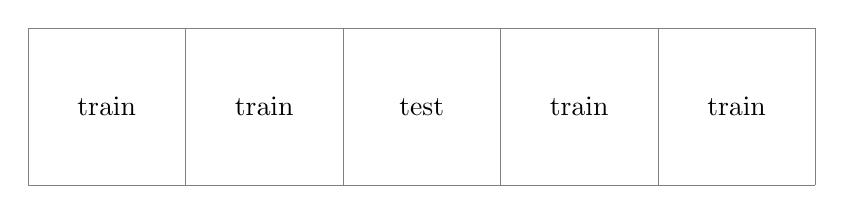
\begin{tikzpicture}
\draw[step=2cm,gray,very thin] (0,0) grid (10,2); 
\draw (5,1) node{test};
\draw (1,1) node{train};
\draw (3,1) node{train};
\draw (7,1) node{train};
\draw (9,1) node{train};
\end{tikzpicture}
\end{center}
\caption{Splitting the data into $K=5$ roughly equal-sized parts.}
\label{fig:KFOLD}
\end{figure}

For the $j^{\mathrm{th}}$ part (third in Figure \ref{fig:KFOLD}), we train the model to the other $K-1$ parts
of the data, and calculate the prediction error of the fitted model when
predicting the $j^{\mathrm{th}}$ part of the data. We repeat this process for $j = \left\lbrace 1,2,\dots,K\right\rbrace$ and
combine the $K$ estimates of prediction error.

Let $\gamma : \left\lbrace 1,\dots,N\right\rbrace\rightarrow  \left\lbrace 1,\dots,K\right\rbrace$ be an indexing
function that indicates the partition to which observation $j$ is allocated by
the randomization. Symbol $\hat{f}_{\boldsymbol{\theta}}^{-j}\left(\boldsymbol{x}\right)$ denotes the fitted model, computed with
the $j^{\mathrm{th}}$th part of the data removed. Then the cross-validation estimate of
prediction error is defined by
\begin{equation}
\mathrm{CV}\left(\hat{f}_{\boldsymbol{\theta}}\right) = \frac{1}{N}\sum_{i = 1}^{N}\mathcal{L}\left(y_i , \hat{f}_{\boldsymbol{\theta}}^{-\gamma\left(i\right)}\left(\boldsymbol{x}_i\right)\right).
\end{equation}
Typical choices of $K$ are 5 or 10 and even case $K = N$ that is known as \emph{leave-one-out} cross--validation. Generally, there is not an universal way of choosing $K$, since it strongly depends on the available number of data. 

The biggest problem of this method is a fact that it is computionally very expensive. For extremely complicated and complex models that are trained for hours or days, is cross--validation inconvenient approach of estimating the prediction error.
\subsection{Akaike information criterion}



\section{Bayesian Inference}
The Bayesian methodology is a well established approach to statistical inference and became very important technique in statistics and data analysis. As its name suggests, Bayesian statistics is based on application of Bayes' rule. In this chapter, we briefly review basic concept of this approach, which was suggested here \cite{smidl}. 

 Let the measured data be denoted by $\mathcal{D}$, defined according to previous section \ref{sec:terminology}. A parametric probabilistic model of the data $\mathcal{D}$ is given by the probability density function  $p(\mathcal{D}|\boldsymbol{\theta})$, where $\boldsymbol{\theta}~\in~\boldsymbol{\Theta}~\subset~\R^s$ denotes parameters of the model. The main idea behind Bayesian theory is the treatment of the unknown parameters $\boldsymbol{\theta}$ as a random variable.  Bayes' rule is applied to infer model parameters $\boldsymbol{\theta}$, therefore
 \begin{equation}\label{Bayesinference}
 	p(\boldsymbol{\theta} | \mathcal{D}) = \frac{p(\boldsymbol{\theta}, \mathcal{D})}{p(\mathcal{D})} = \frac{p(\mathcal{D}| \boldsymbol{\theta})p(\boldsymbol{\theta})}{\int_{\boldsymbol{\Theta}}p(\mathcal{D}|\boldsymbol{\theta})p(\boldsymbol{\theta})\d\boldsymbol{\theta}}.
 \end{equation} 
Since $p(\mathcal{D})$ is just the normalization constant, Equation \eqref{Bayesinference} is often simplified to
\begin{equation}
	p(\boldsymbol{\theta} | \mathcal{D}) \propto p(\mathcal{D}| \boldsymbol{\theta})p(\boldsymbol{\theta}).
\end{equation} 
Symbol $\propto$ means equal up to the normalization constant. The term $p(\boldsymbol{\theta} | \mathcal{D})$ is known as the \emph{posterior} distribution, $p(\mathcal{D}| \boldsymbol{\theta})$  as the \emph{observation model}, and $p(\boldsymbol{\theta})$ is called the \emph{prior} distribution of the $\boldsymbol{\theta}$. Note that evaluation of the normalization constant can be computionally expensive, in higher dimension even intractable. 

Popular choices for an optimal value of the point estimate are:
\begin{enumerate}
	\item Maximum A posteriori estimate (MAP)
	\begin{equation}
		\widehat{\boldsymbol{\theta}}_{\mathrm{MAP}} = \argmax_{\boldsymbol{\theta}} p(\boldsymbol{\theta} | \mathcal{D})
	\end{equation}
This method estimates $\boldsymbol{\theta}$ as the mode of the posterior distribution. It appears to be computionally attractive, as it is not necessary to evaluate the normalization constant. 
\item Mean or expected value
\begin{equation}
	\widehat{\boldsymbol{\theta}}_{\mathrm{B}} = \int_{\boldsymbol{\Theta}} \boldsymbol{\theta}~ p(\boldsymbol{\theta} | \mathcal{D}) \d\boldsymbol{\theta} = \E_{\boldsymbol{\theta} \sim p(\boldsymbol{\theta} | \mathcal{D}) }\left[\boldsymbol{\theta} \right]
\end{equation}
Mean value, unlike MAP estimate, may be very expensive to compute because of the required integration. This may lead to further approximations such as EM algorithm \cite{EM}.
\end{enumerate}	

\subsection{Choice of prior distribution}
For the posterior computation, it is necessary to specify the prior distribution $p(\boldsymbol{\theta})$, unfortunately, this might not be easily determined. This can be achieved via knowledge of previous models, expert knowledge, their combination or even uncertainty about $\boldsymbol{\theta}$ can be viable option. 

There is also many practical aspects of priors:
\begin{itemize}
	\item Regularization - supplementing the data, if there is insufficient data or poorly defined model. 
	\item Imposing various restrictions on the parameters $\boldsymbol{\theta}$ reflecting physical constraints. The choice of prior distribution with bounded support will result to posterior distribution with bounded support as well. 
	\item Non--informative prior - if the data are informative enough to make a prediction, it is proposed to choose a prior with minimal impact on the posterior distribution, such as uniform distribution. However, typical choices of non--informative priors are so--called \emph{Jeffreys priors} \cite{jeffrey}.
\end{itemize}



\subsection{Prediction}
We are not usually interested in the value of $\widehat{\boldsymbol{\theta}}$ itself but rather, once the model is estimated, we are interested in making prediction of output variable $y^{\star}$ for the new input variable $\boldsymbol{x}^{\star}$. Note that the symbol $\mathcal{D}$ contains all of the previous given data $\boldsymbol{x}$ and $y$. The posterior predictive distribution is then determined by distribution of the $y^{\star}$, marginalized over the posterior
\begin{equation}
	p(y^{\star} | \boldsymbol{x}^{\star}, \mathcal{D}) =   \int_{\boldsymbol{\Theta}} p(y^{\star}|\boldsymbol{x}^{\star}, \boldsymbol{\theta}) p(\boldsymbol{\theta}|\mathcal{D}) \d\boldsymbol{\theta}.
\end{equation} 
When the distribution $p(\boldsymbol{\theta}|\mathcal{D})$ is not available, we have to approximate leveraging the Dirac delta function $\delta(x)$  
\begin{equation}
p(y^{\star} | \boldsymbol{x}^{\star}, \mathcal{D}) = \int_{\boldsymbol{\Theta}} 	p(y^{\star}|\boldsymbol{x}^{\star}, \boldsymbol{\theta}) \delta(\boldsymbol{\theta} - \widehat{\boldsymbol{\theta}})\d\boldsymbol{\theta} = p(y^{\star}|\boldsymbol{x}^{\star}, \widehat{\boldsymbol{\theta}}),
\end{equation}
causing an error. In typical MAP, this is known as \emph{over--fitting}. Prediction error is then defined by a loss function measuring errors between $y$ and $\widehat{y}$
\begin{equation}
	\mathrm{Err} = \pazocal{L}\left(\widehat{y}, y \right),
\end{equation}	
where $\widehat{y} = \widehat{f}_{\boldsymbol{\theta}}\left(\boldsymbol{x}\right) = f(\widehat{\boldsymbol{\theta}}, \boldsymbol{x})$.  As an example, we can mention couple of typically used loss functions 
\begin{equation}
\pazocal{L}\left(y,\widehat{y} \right) =
 \begin{cases}
	 \left(y - \widehat{y}\right)^2& \text{squared error}\\
	 \abs{y - \widehat{y}} & \text{absolute error}\\
\end{cases}   .
\end{equation}
We shall also discuss the problem of the model complexity. Consider a polynomial regression problem,  where the model is defined by
\begin{equation}
	f_{\boldsymbol{\theta}}(x) = \sum_{i=0}^{s-1}\theta_ix^i.
\end{equation}
 Here, over--fitting occurs very frequently. Model complexity of this case is very intuitive, as it is just the order of the polynomial, $s-1$.  Smaller orders of the polynomial (may) give rather poor fits to the data in contrast to much higher order polynomial giving an excellent fit. Such polynomial passes exactly through each datapoint, however, oscillates wildly and gives poor prediction for new input variable $x^{\star}$. \\
To obtain some quantitative insight into dependence of the generalization performance on model complexity, consider separate test set of data (testing data) used to assess the performance of the model. 
In general, prediction error evaluated on the training data for increasing model complexity approaches zero. On the other hand, prediction error evaluated on the testing data for increasing model complexity is (from certain point) increasing as well. The typical scenario is illustrated in Figure \ref{fig:Prediction_error}.
 \begin{figure}[h]
	\centering
	\includegraphics[width=16.0cm]{plots/Images/PE3.pdf}
	\caption{Evaluation of prediction error as a function of model complexity.}%
	\label{fig:Prediction_error}%
\end{figure}


 
